\chapter{\IfLanguageName{dutch}{Stand van zaken}{State of the art}}%
\label{ch:stand-van-zaken}

In dit onderdeel wordt dieper ingegaan op wat flutter is hoe het werkt. Daarna wordt er onderzocht welke state management benaderingen er 
zijn en hoe ze werken en worden ze met elkaar vergeleken.

\section{{Flutter}}%
\label{sec:Flutter}
Flutter is een open-source framework ontwikkeld door Google coor het bouwen van multi-platform applicaties vanuit één codebase. 
Dit betekent dus dat ontwikkelaars in een korte tijd applicaties kunnen ontwikkelen voor mobiele, web, desktop en ook voor embedded systemen.
Bovendien wordt flutter code vertaald naar native machine code, wat zorgt voor snelle applicaties en annimaties. \footnote{\url{https://flutter.dev}}
\\
\\
Flutter applicaties worden geschreven met Dart, een programmeertaal die ook eigendom is van Google. Dart ondersteunt AOT (ahead of time) 
compilation en JIT (just in time) compilation. AOT verbetert de opstarttijd en performantie van de application en dankzij JIT compilation 
wordt hot reload mogelijk. Dit wilt zeggen dat enkel de gewijzigd stukken code opnieuw moet gecompileerd worden in plaats van de volledige applicatie.
Het is dus mogelijk om wijziginen in bijna real time te testen. \footnote{\url{https://docs.dart.dev}}

\section{Flutter Architectuur}
\label{sec:Flutter Architectuur}
Voor dat er over de state management binnen flutter besproken kan worden, wordt er eerst een paar begrippen uitgelegd binnen Flutter. Ook wordt er in dit deel
uitgelegd hoe Flutter werkt intern.

\subsection[widget]{Widgets}
\label{sec:Widgets}
In Flutter wordt alle componenten in de app als "Widget" beschouwd. Wat een widget is is eigenlijk een Dart klasse die beschrijft hoe een stuk van de user interface eruit ziet.
De UI van de app wordt dus met andere worden gebouwd door widgets in ouder-kind relatie te combineren. Elk widget wordt in een parent widget genest en context kan doorgegeven worden van ouder naar kind.
Alle widgets zitten dus in een widget boom, met elk ouder widget één of meerdere kind widgets.
\\
\begin{figure}[h]
    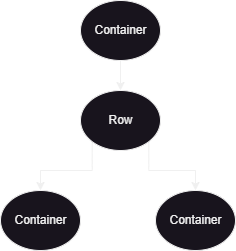
\includegraphics{graphics/widgetTree.png}
    \caption{Voorbeeld van een widget boom}
\end{figure}
\\
%TODO: add piece of code block for widget tree
Elk widget is onderanderlijk. Applicaties werken hun ui bij als reactie op gebeurtenissen (zoals een gebruikersinteractie) door het framework te vertellen 
dat een widet in de hiërarchie te vervangen door een andere widget. De ouder widgets worden met de nieuwe vergeleken door het framework en wordt de 
gebruikersinterface efficiënt bijgewerkt.


\subsection[states]{States}
\label{sec:States}
Elk widget kan states hebben. Flutter beschrijft een state als informatie die enerzijds synchroon kan worden gelezen wanneer de widget wordt gebouwd en anderzijds
kan veranderen tijdens de levensduur van de widget.  \footnote{\url{https://api.flutter.dev/flutter/widgets/State-class.html}}


\subsection[widget states]{Widget states}
\label{sec:Widget states}
Nu dat er een beeld is over wat states zijn binnen Flutter, kan er over de 2 meest gebruikte soorten widgets besproken worden. 
 \begin{itemize}
     \item stateless widget
     \item stateful widget
 \end{itemize}

\section{{State management}}%
\label{sec:State management}
Zoals eerder vermeld wordt Flutter ontwikkeld om performant te zijn. Maar een mogelijke reden die de performantie van de applicatie kan beïnvloeden is het slecht 
bijhouden van states binnen de applicatie.
\\
State management is een techniek, of meerdere, die gebruikt wordt om veranderingen in de applicatie te beheren. Het gebruik van de juiste state management kan zorgen 
voor betere leesbaarheid van code en ook voor een performanter applicatie. 
\subsection{{setState}}%
\label{sec:setState}
todo
\\
\subsection{{Provider}}%
\label{sec:Provider}
todo
\\
\subsection{{RiverPod}}%
\label{sec:RiverPod}
todo
\\
\subsection{{GetX}}%
\label{sec:GetX}
todo
\\
\subsection{{Redux}}%
\label{sec:Redux}
todo
\\
\subsection{{Bloc}}%
\label{sec:Bloc}
todo
\\
\subsection{{MobX}}%
\label{sec:MobX}
todo
% Tip: Begin elk hoofdstuk met een paragraaf inleiding die beschrijft hoe
% dit hoofdstuk past binnen het geheel van de bachelorproef. Geef in het
% bijzonder aan wat de link is met het vorige en volgende hoofdstuk.

% Pas na deze inleidende paragraaf komt de eerste sectiehoofding.

%Dit hoofdstuk bevat je literatuurstudie. De inhoud gaat verder op de inleiding, maar zal het onderwerp van de bachelorproef *diepgaand* uitspitten. De bedoeling is dat de lezer na lezing van dit hoofdstuk helemaal op de hoogte is van de huidige stand van zaken (state-of-the-art) in het onderzoeksdomein. Iemand die niet vertrouwd is met het onderwerp, weet nu voldoende om de rest van het verhaal te kunnen volgen, zonder dat die er nog andere informatie moet over opzoeken \autocite{Pollefliet2011}.

%Je verwijst bij elke bewering die je doet, vakterm die je introduceert, enz.\ naar je bronnen. In \LaTeX{} kan dat met het commando \texttt{$\backslash${textcite\{\}}} of \texttt{$\backslash${autocite\{\}}}. Als argument van het commando geef je de ``sleutel'' van een ``record'' in een bibliografische databank in het Bib\LaTeX{}-formaat (een tekstbestand). Als je expliciet naar de auteur verwijst in de zin (narratieve referentie), gebruik je \texttt{$\backslash${}textcite\{\}}. Soms is de auteursnaam niet expliciet een onderdeel van de zin, dan gebruik je \texttt{$\backslash${}autocite\{\}} (referentie tussen haakjes). Dit gebruik je bv.~bij een citaat, of om in het bijschrift van een overgenomen afbeelding, broncode, tabel, enz. te verwijzen naar de bron. In de volgende paragraaf een voorbeeld van elk.

%\textcite{Knuth1998} schreef een van de standaardwerken over sorteer- en zoekalgoritmen. Experten zijn het erover eens dat cloud computing een interessante opportuniteit vormen, zowel voor gebruikers als voor dienstverleners op vlak van informatietechnologie~\autocite{Creeger2009}.

%Let er ook op: het \texttt{cite}-commando voor de punt, dus binnen de zin. Je verwijst meteen naar een bron in de eerste zin die erop gebaseerd is, dus niet pas op het einde van een paragraaf.


